\chapter{Theory of Sentence Embeddings}
\label{appendix:embedding-theory}

This appendix expands on the theoretical and practical foundations of sentence embeddings. These representations serve as the basis for semantic similarity throughout the system, as discussed in Chapter~\ref{chapter:embedding}. Understanding how they are constructed and used is essential for grasping the logic behind embedding-based search and classification.

\section{From Words to Vectors}
In traditional NLP, words are first tokenized and represented numerically. Early methods like one-hot encoding fail to capture semantic relationships between words. This motivated the development of distributed representations — where words are embedded in continuous vector spaces.

Word embeddings like Word2Vec~\parencite{mikolov2013efficient} and GloVe~\parencite{pennington2014glove} map words with similar contexts to nearby points in a high-dimensional space. However, they produce static embeddings: the word "bank" will have the same vector whether referring to a financial institution or a riverbank.

\section{Sentence Embeddings}
Sentence embeddings aim to extend this idea to whole sentences or paragraphs. They encode variable-length text into fixed-length dense vectors that capture meaning, context, and structure.

Formally, let:
\[
f(t) = \vec{v}, \quad \vec{v} \in \mathbb{R}^d
\]
where \( t \) is the input sentence, \( f \) is an embedding function (typically a neural model), and \( d \) is the dimensionality of the embedding space.

\section{Transformer-Based Embeddings}
Transformer models~\parencite{vaswani2017attention} have become the backbone of modern NLP. Instead of relying on fixed context windows, they use self-attention to consider the entire sentence when encoding each word.

Sentence-BERT (SBERT)~\parencite{reimers2019sentencebert} fine-tunes transformer architectures to generate sentence-level embeddings. This project uses the distilled variant \texttt{all-MiniLM-L6-v2}, which balances semantic performance with CPU efficiency.

\subsection*{Architecture Overview}
Below is a simplified diagram of the embedding process using a transformer:

\begin{figure}[H]
\centering
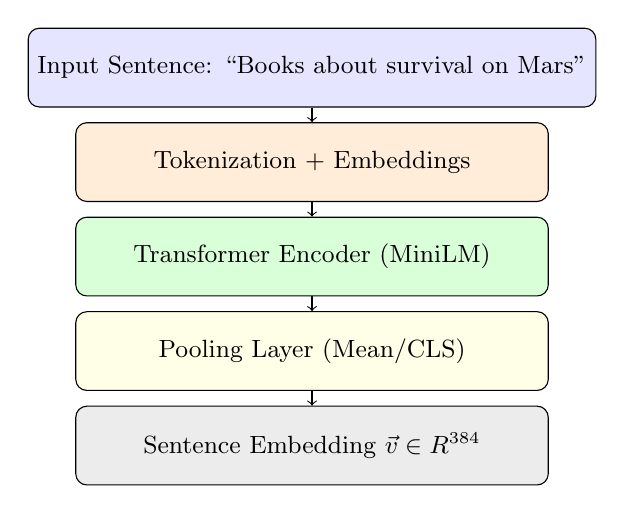
\begin{tikzpicture}[node distance=1.2cm, every node/.style={font=\small}]
    \node (input) [draw, rounded corners, minimum width=6cm, minimum height=1cm, fill=blue!10] {Input Sentence: ``Books about survival on Mars''};

    \node (tokens) [below of=input, draw, rounded corners, minimum width=6cm, minimum height=1cm, fill=orange!15] {Tokenization + Embeddings};

    \node (transformer) [below of=tokens, draw, rounded corners, minimum width=6cm, minimum height=1cm, fill=green!15] {Transformer Encoder (MiniLM)};

    \node (pooling) [below of=transformer, draw, rounded corners, minimum width=6cm, minimum height=1cm, fill=yellow!10] {Pooling Layer (Mean/CLS)};

    \node (vector) [below of=pooling, draw, rounded corners, minimum width=6cm, minimum height=1cm, fill=gray!15] {Sentence Embedding \( \vec{v} \in \mathbb{R}^{384} \)};

    \draw[->] (input) -- (tokens);
    \draw[->] (tokens) -- (transformer);
    \draw[->] (transformer) -- (pooling);
    \draw[->] (pooling) -- (vector);
\end{tikzpicture}
\caption{Pipeline for generating a sentence embedding}
\end{figure}

\section{Similarity Measures}
Once embedded, sentences can be compared using vector similarity. Common measures include:

\begin{itemize}
    \item \textbf{Cosine similarity:} 
    \[
    \cos(\theta) = \frac{\vec{v}_1 \cdot \vec{v}_2}{\|\vec{v}_1\| \|\vec{v}_2\|}
    \]
    Measures the angle between two vectors, emphasizing direction over magnitude.

    \item \textbf{Euclidean (L2) distance:}
    \[
    \|\vec{v}_1 - \vec{v}_2\|_2^2
    \]
    Measures straight-line distance. This project uses L2 distance for compatibility with FAISS.
\end{itemize}

\section{Intuitive Example}
Consider these two sentences:

\begin{quote}
\emph{``A man is walking a dog.''} \\
\emph{``Someone strolls through the park with a pet.''}
\end{quote}

Despite having no identical words, their embeddings lie close together in semantic space, enabling meaningful comparisons beyond keyword overlap.

\section{Limitations and Challenges}
While powerful, sentence embeddings have limitations:

\begin{itemize}
    \item Cannot perfectly disambiguate sarcasm, irony, or negation
    \item Performance degrades on domain-specific jargon
    \item Quality depends heavily on description clarity and length
\end{itemize}

\section{Conclusion}
Sentence embeddings are a foundational tool for semantic search and classification. By transforming language into geometry, they unlock flexible, content-aware systems that work without user histories or explicit labels.

Models like MiniLM make such capabilities available even on modest hardware — aligning with the project's offline-first design.

